%====================================================================================
\section[Pareto]{Condiciones del óptimo de Pareto}
%====================================================================================

\begin{frame}{Óptimo de Pareto}
	Asignación eficiente: las curvas de indiferencia de los dos consumidores tienen que ser tangentes. De no ser así, siempre se podría mejorar a un agente sin empeorar al otro.\\
	
	Condición necesaria para la eficiencia (en una solución interior): condición de \textbf{eficiencia asignativa del consumo}:
		$$RMS_{x_1,x_2}^{A}(x_{1}^{A},x_{2}^{A})=RMS_{x_1,x_2}^{B}(x_{1}^{B},x_{2}^{B})$$
\end{frame}
%------------------------------------------------
\begin{frame}{Óptimo de Pareto}
	Resolviendo el problema de optimización
		\begin{align*}
			& \text{Max } \quad u^{A}\left(x_{1}^{A},x_{2}^{A}\right) \\
			& \begin{array}{ll}
				\text{s.a: } & u^{B}\left(x_{1}^{B},x_{2}^{B} \right) = \overline{u}^{B}\\
				& x_{1}^{A}+x_{1}^{B} = \overline{w}_1  \\
				& x_{2}^{A}+x_{2}^{B} = \overline{w}_2  
			\end{array}
		\end{align*}
	Langrangiano:\\
	{\small $$\mathscr{L} = u^{A}\left( x_{1}^{A},x_{2}^{A}\right)  + \lambda \left[u^{B}(x_{1}^{B},x_{2}^{B}) - \overline{u}^{B}\right] +\mu_{x_1}\left[\overline{w}_1-x_{1}^{A}-x_{1}^{B} \right] +\mu_{x_2}\left[\overline{w}_2-x_{2}^{A}-x_{2}^{B}\right]$$}
\end{frame}
%------------------------------------------------
\begin{frame}{Óptimo de Pareto}
	Condiciones de primer orden
		$$	\left.
				\begin{array}{l}
					\frac{\partial \mathscr{L}}{\partial x_{1}^{A}}=\frac{\partial u^{A}\left( x_{1}^{A},x_{2}^{A}\right)}{\partial x_{1}^{A}}-\mu_{x_1}=0 \\ [.5cm]
					\frac{\partial \mathscr{L}}{\partial x_{2}^{A}}=\frac{\partial u^{A}\left( x_{1}^{A},x_{2}^{A}\right)}{\partial x_{2}^{A}}-\mu_{x_2}=0
				\end{array}
			\right\} \Rightarrow \frac{\frac{\partial u^{A}\left( x_{1}^{A},x_{2}^{A}\right)}{\partial x_{1}^{A}}}{\frac{\partial u^{A}\left( x_{1}^{A},x_{2}^{A}\right)}{\partial x_{2}^{A}}}=RMS_{x_1,x_2}^{A}\left( x_{1}^{A},x_{2}^{A}\right)=\frac{\mu_{x_1}}{\mu_{x_2}}$$
		\bigskip
		$$	\left.
				\begin{array}{l}
					\frac{\partial \mathscr{L}}{\partial x_{1}^{B}}=\lambda \frac{\partial u^{B}\left( x_{1}^{B},x_{2}^{B}\right)}{\partial x_{1}^{B}}-\mu_{x_1}=0 \\  [.5cm]
					\frac{\partial \mathscr{L}}{\partial x_{2}^{B}}=\lambda \frac{\partial u^{B}\left( x_{1}^{B},x_{2}^{B}\right)}{\partial x_{2}^{B}}-\mu_{x_2}=0
				\end{array}
			\right\} \Rightarrow \frac{\lambda \frac{\partial u^{B}\left( x_{1}^{B},x_{2}^{B}\right)}{\partial x_{1}^{B}}}{\lambda\frac{\partial u^{B}\left( x_{1}^{B},x_{2}^{B}\right)}{\partial x_{2}^{B}}}=RMS_{x_1,x_2}^{B}\left( x_{1}^{B},x_{2}^{B}\right)=\frac{\mu_{x_1}}{\mu_{x_2}}$$
		\bigskip
		$$	\left.
				\begin{array}{l}
					RMS_{x_1,x_2}^{A}\left( x_{1}^{A},x_{2}^{A}\right)=\frac{\mu_{x_1}}{\mu_{x_2}}\\  [.5cm]
					RMS_{x_1,x_2}^{B}\left( x_{1}^{B},x_{2}^{B}\right)=\frac{\mu_{x_1}}{\mu_{x_2}}
				\end{array}
			\right\} \Rightarrow RMS_{x_1,x_2}^{A}\left( x_{1}^{A},x_{2}^{A}\right) = RMS_{x_1,x_2}^{B}\left( x_{1}^{B},x_{2}^{B}\right)$$
\end{frame}
%------------------------------------------------
\begin{frame}{Curva de contrato}
		\begin{figure}
			\centering
			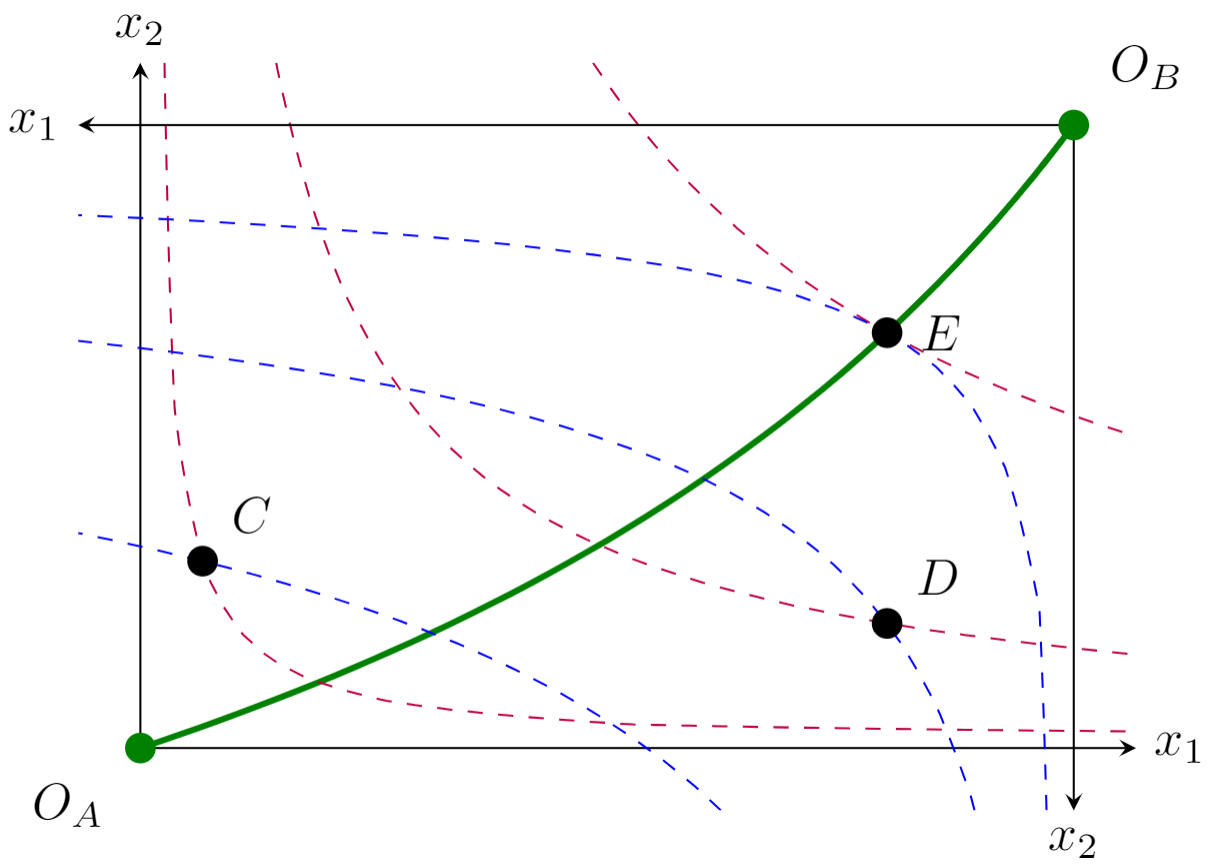
\includegraphics[width = \linewidth]{figures/pic_13}
		\end{figure}
\end{frame}